\documentclass[11pt]{article}
\usepackage[T2A]{fontenc}
\usepackage[utf8]{inputenc}
\usepackage[english,russian]{babel}
    \usepackage[breakable]{tcolorbox}
    \usepackage{parskip} % Stop auto-indenting (to mimic markdown behaviour)
    

    % Basic figure setup, for now with no caption control since it's done
    % automatically by Pandoc (which extracts ![](path) syntax from Markdown).
    \usepackage{graphicx}
    % Maintain compatibility with old templates. Remove in nbconvert 6.0
    \let\Oldincludegraphics\includegraphics
    % Ensure that by default, figures have no caption (until we provide a
    % proper Figure object with a Caption API and a way to capture that
    % in the conversion process - todo).
    \usepackage{caption}
    \DeclareCaptionFormat{nocaption}{}
    \captionsetup{format=nocaption,aboveskip=0pt,belowskip=0pt}

    \usepackage{float}
    \floatplacement{figure}{H} % forces figures to be placed at the correct location
    \usepackage{xcolor} % Allow colors to be defined
    \usepackage{enumerate} % Needed for markdown enumerations to work
    \usepackage{geometry} % Used to adjust the document margins
    \usepackage{amsmath} % Equations
    \usepackage{amssymb} % Equations
    \usepackage{textcomp} % defines textquotesingle
    % Hack from http://tex.stackexchange.com/a/47451/13684:
    \AtBeginDocument{%
        \def\PYZsq{\textquotesingle}% Upright quotes in Pygmentized code
    }
    \usepackage{upquote} % Upright quotes for verbatim code
    \usepackage{eurosym} % defines \euro

    \usepackage{iftex}
    \ifPDFTeX
        \usepackage[T1]{fontenc}
        \IfFileExists{alphabeta.sty}{
              \usepackage{alphabeta}
          }{
              \usepackage[mathletters]{ucs}
              \usepackage[utf8x]{inputenc}
          }
    \else
        \usepackage{fontspec}
        \usepackage{unicode-math}
    \fi

    \usepackage{fancyvrb} % verbatim replacement that allows latex
    \usepackage{grffile} % extends the file name processing of package graphics
                         % to support a larger range
    \makeatletter % fix for old versions of grffile with XeLaTeX
    \@ifpackagelater{grffile}{2019/11/01}
    {
      % Do nothing on new versions
    }
    {
      \def\Gread@@xetex#1{%
        \IfFileExists{"\Gin@base".bb}%
        {\Gread@eps{\Gin@base.bb}}%
        {\Gread@@xetex@aux#1}%
      }
    }
    \makeatother
    \usepackage[Export]{adjustbox} % Used to constrain images to a maximum size
    \adjustboxset{max size={0.9\linewidth}{0.9\paperheight}}

    % The hyperref package gives us a pdf with properly built
    % internal navigation ('pdf bookmarks' for the table of contents,
    % internal cross-reference links, web links for URLs, etc.)
    \usepackage{hyperref}
    % The default LaTeX title has an obnoxious amount of whitespace. By default,
    % titling removes some of it. It also provides customization options.
    \usepackage{titling}
    \usepackage{longtable} % longtable support required by pandoc >1.10
    \usepackage{booktabs}  % table support for pandoc > 1.12.2
    \usepackage{array}     % table support for pandoc >= 2.11.3
    \usepackage{calc}      % table minipage width calculation for pandoc >= 2.11.1
    \usepackage[inline]{enumitem} % IRkernel/repr support (it uses the enumerate* environment)
    \usepackage[normalem]{ulem} % ulem is needed to support strikethroughs (\sout)
                                % normalem makes italics be italics, not underlines
    \usepackage{mathrsfs}
    

    
    % Colors for the hyperref package
    \definecolor{urlcolor}{rgb}{0,.145,.698}
    \definecolor{linkcolor}{rgb}{.71,0.21,0.01}
    \definecolor{citecolor}{rgb}{.12,.54,.11}

    % ANSI colors
    \definecolor{ansi-black}{HTML}{3E424D}
    \definecolor{ansi-black-intense}{HTML}{282C36}
    \definecolor{ansi-red}{HTML}{E75C58}
    \definecolor{ansi-red-intense}{HTML}{B22B31}
    \definecolor{ansi-green}{HTML}{00A250}
    \definecolor{ansi-green-intense}{HTML}{007427}
    \definecolor{ansi-yellow}{HTML}{DDB62B}
    \definecolor{ansi-yellow-intense}{HTML}{B27D12}
    \definecolor{ansi-blue}{HTML}{208FFB}
    \definecolor{ansi-blue-intense}{HTML}{0065CA}
    \definecolor{ansi-magenta}{HTML}{D160C4}
    \definecolor{ansi-magenta-intense}{HTML}{A03196}
    \definecolor{ansi-cyan}{HTML}{60C6C8}
    \definecolor{ansi-cyan-intense}{HTML}{258F8F}
    \definecolor{ansi-white}{HTML}{C5C1B4}
    \definecolor{ansi-white-intense}{HTML}{A1A6B2}
    \definecolor{ansi-default-inverse-fg}{HTML}{FFFFFF}
    \definecolor{ansi-default-inverse-bg}{HTML}{000000}

    % common color for the border for error outputs.
    \definecolor{outerrorbackground}{HTML}{FFDFDF}

    % commands and environments needed by pandoc snippets
    % extracted from the output of `pandoc -s`
    \providecommand{\tightlist}{%
      \setlength{\itemsep}{0pt}\setlength{\parskip}{0pt}}
    \DefineVerbatimEnvironment{Highlighting}{Verbatim}{commandchars=\\\{\}}
    % Add ',fontsize=\small' for more characters per line
    \newenvironment{Shaded}{}{}
    \newcommand{\KeywordTok}[1]{\textcolor[rgb]{0.00,0.44,0.13}{\textbf{{#1}}}}
    \newcommand{\DataTypeTok}[1]{\textcolor[rgb]{0.56,0.13,0.00}{{#1}}}
    \newcommand{\DecValTok}[1]{\textcolor[rgb]{0.25,0.63,0.44}{{#1}}}
    \newcommand{\BaseNTok}[1]{\textcolor[rgb]{0.25,0.63,0.44}{{#1}}}
    \newcommand{\FloatTok}[1]{\textcolor[rgb]{0.25,0.63,0.44}{{#1}}}
    \newcommand{\CharTok}[1]{\textcolor[rgb]{0.25,0.44,0.63}{{#1}}}
    \newcommand{\StringTok}[1]{\textcolor[rgb]{0.25,0.44,0.63}{{#1}}}
    \newcommand{\CommentTok}[1]{\textcolor[rgb]{0.38,0.63,0.69}{\textit{{#1}}}}
    \newcommand{\OtherTok}[1]{\textcolor[rgb]{0.00,0.44,0.13}{{#1}}}
    \newcommand{\AlertTok}[1]{\textcolor[rgb]{1.00,0.00,0.00}{\textbf{{#1}}}}
    \newcommand{\FunctionTok}[1]{\textcolor[rgb]{0.02,0.16,0.49}{{#1}}}
    \newcommand{\RegionMarkerTok}[1]{{#1}}
    \newcommand{\ErrorTok}[1]{\textcolor[rgb]{1.00,0.00,0.00}{\textbf{{#1}}}}
    \newcommand{\NormalTok}[1]{{#1}}

    % Additional commands for more recent versions of Pandoc
    \newcommand{\ConstantTok}[1]{\textcolor[rgb]{0.53,0.00,0.00}{{#1}}}
    \newcommand{\SpecialCharTok}[1]{\textcolor[rgb]{0.25,0.44,0.63}{{#1}}}
    \newcommand{\VerbatimStringTok}[1]{\textcolor[rgb]{0.25,0.44,0.63}{{#1}}}
    \newcommand{\SpecialStringTok}[1]{\textcolor[rgb]{0.73,0.40,0.53}{{#1}}}
    \newcommand{\ImportTok}[1]{{#1}}
    \newcommand{\DocumentationTok}[1]{\textcolor[rgb]{0.73,0.13,0.13}{\textit{{#1}}}}
    \newcommand{\AnnotationTok}[1]{\textcolor[rgb]{0.38,0.63,0.69}{\textbf{\textit{{#1}}}}}
    \newcommand{\CommentVarTok}[1]{\textcolor[rgb]{0.38,0.63,0.69}{\textbf{\textit{{#1}}}}}
    \newcommand{\VariableTok}[1]{\textcolor[rgb]{0.10,0.09,0.49}{{#1}}}
    \newcommand{\ControlFlowTok}[1]{\textcolor[rgb]{0.00,0.44,0.13}{\textbf{{#1}}}}
    \newcommand{\OperatorTok}[1]{\textcolor[rgb]{0.40,0.40,0.40}{{#1}}}
    \newcommand{\BuiltInTok}[1]{{#1}}
    \newcommand{\ExtensionTok}[1]{{#1}}
    \newcommand{\PreprocessorTok}[1]{\textcolor[rgb]{0.74,0.48,0.00}{{#1}}}
    \newcommand{\AttributeTok}[1]{\textcolor[rgb]{0.49,0.56,0.16}{{#1}}}
    \newcommand{\InformationTok}[1]{\textcolor[rgb]{0.38,0.63,0.69}{\textbf{\textit{{#1}}}}}
    \newcommand{\WarningTok}[1]{\textcolor[rgb]{0.38,0.63,0.69}{\textbf{\textit{{#1}}}}}


    % Define a nice break command that doesn't care if a line doesn't already
    % exist.
    \def\br{\hspace*{\fill} \\* }
    % Math Jax compatibility definitions
    \def\gt{>}
    \def\lt{<}
    \let\Oldtex\TeX
    \let\Oldlatex\LaTeX
    \renewcommand{\TeX}{\textrm{\Oldtex}}
    \renewcommand{\LaTeX}{\textrm{\Oldlatex}}
    % Document parameters
    % Document title
    \title{6}
    
    
    
    
    
% Pygments definitions
\makeatletter
\def\PY@reset{\let\PY@it=\relax \let\PY@bf=\relax%
    \let\PY@ul=\relax \let\PY@tc=\relax%
    \let\PY@bc=\relax \let\PY@ff=\relax}
\def\PY@tok#1{\csname PY@tok@#1\endcsname}
\def\PY@toks#1+{\ifx\relax#1\empty\else%
    \PY@tok{#1}\expandafter\PY@toks\fi}
\def\PY@do#1{\PY@bc{\PY@tc{\PY@ul{%
    \PY@it{\PY@bf{\PY@ff{#1}}}}}}}
\def\PY#1#2{\PY@reset\PY@toks#1+\relax+\PY@do{#2}}

\@namedef{PY@tok@w}{\def\PY@tc##1{\textcolor[rgb]{0.73,0.73,0.73}{##1}}}
\@namedef{PY@tok@c}{\let\PY@it=\textit\def\PY@tc##1{\textcolor[rgb]{0.24,0.48,0.48}{##1}}}
\@namedef{PY@tok@cp}{\def\PY@tc##1{\textcolor[rgb]{0.61,0.40,0.00}{##1}}}
\@namedef{PY@tok@k}{\let\PY@bf=\textbf\def\PY@tc##1{\textcolor[rgb]{0.00,0.50,0.00}{##1}}}
\@namedef{PY@tok@kp}{\def\PY@tc##1{\textcolor[rgb]{0.00,0.50,0.00}{##1}}}
\@namedef{PY@tok@kt}{\def\PY@tc##1{\textcolor[rgb]{0.69,0.00,0.25}{##1}}}
\@namedef{PY@tok@o}{\def\PY@tc##1{\textcolor[rgb]{0.40,0.40,0.40}{##1}}}
\@namedef{PY@tok@ow}{\let\PY@bf=\textbf\def\PY@tc##1{\textcolor[rgb]{0.67,0.13,1.00}{##1}}}
\@namedef{PY@tok@nb}{\def\PY@tc##1{\textcolor[rgb]{0.00,0.50,0.00}{##1}}}
\@namedef{PY@tok@nf}{\def\PY@tc##1{\textcolor[rgb]{0.00,0.00,1.00}{##1}}}
\@namedef{PY@tok@nc}{\let\PY@bf=\textbf\def\PY@tc##1{\textcolor[rgb]{0.00,0.00,1.00}{##1}}}
\@namedef{PY@tok@nn}{\let\PY@bf=\textbf\def\PY@tc##1{\textcolor[rgb]{0.00,0.00,1.00}{##1}}}
\@namedef{PY@tok@ne}{\let\PY@bf=\textbf\def\PY@tc##1{\textcolor[rgb]{0.80,0.25,0.22}{##1}}}
\@namedef{PY@tok@nv}{\def\PY@tc##1{\textcolor[rgb]{0.10,0.09,0.49}{##1}}}
\@namedef{PY@tok@no}{\def\PY@tc##1{\textcolor[rgb]{0.53,0.00,0.00}{##1}}}
\@namedef{PY@tok@nl}{\def\PY@tc##1{\textcolor[rgb]{0.46,0.46,0.00}{##1}}}
\@namedef{PY@tok@ni}{\let\PY@bf=\textbf\def\PY@tc##1{\textcolor[rgb]{0.44,0.44,0.44}{##1}}}
\@namedef{PY@tok@na}{\def\PY@tc##1{\textcolor[rgb]{0.41,0.47,0.13}{##1}}}
\@namedef{PY@tok@nt}{\let\PY@bf=\textbf\def\PY@tc##1{\textcolor[rgb]{0.00,0.50,0.00}{##1}}}
\@namedef{PY@tok@nd}{\def\PY@tc##1{\textcolor[rgb]{0.67,0.13,1.00}{##1}}}
\@namedef{PY@tok@s}{\def\PY@tc##1{\textcolor[rgb]{0.73,0.13,0.13}{##1}}}
\@namedef{PY@tok@sd}{\let\PY@it=\textit\def\PY@tc##1{\textcolor[rgb]{0.73,0.13,0.13}{##1}}}
\@namedef{PY@tok@si}{\let\PY@bf=\textbf\def\PY@tc##1{\textcolor[rgb]{0.64,0.35,0.47}{##1}}}
\@namedef{PY@tok@se}{\let\PY@bf=\textbf\def\PY@tc##1{\textcolor[rgb]{0.67,0.36,0.12}{##1}}}
\@namedef{PY@tok@sr}{\def\PY@tc##1{\textcolor[rgb]{0.64,0.35,0.47}{##1}}}
\@namedef{PY@tok@ss}{\def\PY@tc##1{\textcolor[rgb]{0.10,0.09,0.49}{##1}}}
\@namedef{PY@tok@sx}{\def\PY@tc##1{\textcolor[rgb]{0.00,0.50,0.00}{##1}}}
\@namedef{PY@tok@m}{\def\PY@tc##1{\textcolor[rgb]{0.40,0.40,0.40}{##1}}}
\@namedef{PY@tok@gh}{\let\PY@bf=\textbf\def\PY@tc##1{\textcolor[rgb]{0.00,0.00,0.50}{##1}}}
\@namedef{PY@tok@gu}{\let\PY@bf=\textbf\def\PY@tc##1{\textcolor[rgb]{0.50,0.00,0.50}{##1}}}
\@namedef{PY@tok@gd}{\def\PY@tc##1{\textcolor[rgb]{0.63,0.00,0.00}{##1}}}
\@namedef{PY@tok@gi}{\def\PY@tc##1{\textcolor[rgb]{0.00,0.52,0.00}{##1}}}
\@namedef{PY@tok@gr}{\def\PY@tc##1{\textcolor[rgb]{0.89,0.00,0.00}{##1}}}
\@namedef{PY@tok@ge}{\let\PY@it=\textit}
\@namedef{PY@tok@gs}{\let\PY@bf=\textbf}
\@namedef{PY@tok@gp}{\let\PY@bf=\textbf\def\PY@tc##1{\textcolor[rgb]{0.00,0.00,0.50}{##1}}}
\@namedef{PY@tok@go}{\def\PY@tc##1{\textcolor[rgb]{0.44,0.44,0.44}{##1}}}
\@namedef{PY@tok@gt}{\def\PY@tc##1{\textcolor[rgb]{0.00,0.27,0.87}{##1}}}
\@namedef{PY@tok@err}{\def\PY@bc##1{{\setlength{\fboxsep}{\string -\fboxrule}\fcolorbox[rgb]{1.00,0.00,0.00}{1,1,1}{\strut ##1}}}}
\@namedef{PY@tok@kc}{\let\PY@bf=\textbf\def\PY@tc##1{\textcolor[rgb]{0.00,0.50,0.00}{##1}}}
\@namedef{PY@tok@kd}{\let\PY@bf=\textbf\def\PY@tc##1{\textcolor[rgb]{0.00,0.50,0.00}{##1}}}
\@namedef{PY@tok@kn}{\let\PY@bf=\textbf\def\PY@tc##1{\textcolor[rgb]{0.00,0.50,0.00}{##1}}}
\@namedef{PY@tok@kr}{\let\PY@bf=\textbf\def\PY@tc##1{\textcolor[rgb]{0.00,0.50,0.00}{##1}}}
\@namedef{PY@tok@bp}{\def\PY@tc##1{\textcolor[rgb]{0.00,0.50,0.00}{##1}}}
\@namedef{PY@tok@fm}{\def\PY@tc##1{\textcolor[rgb]{0.00,0.00,1.00}{##1}}}
\@namedef{PY@tok@vc}{\def\PY@tc##1{\textcolor[rgb]{0.10,0.09,0.49}{##1}}}
\@namedef{PY@tok@vg}{\def\PY@tc##1{\textcolor[rgb]{0.10,0.09,0.49}{##1}}}
\@namedef{PY@tok@vi}{\def\PY@tc##1{\textcolor[rgb]{0.10,0.09,0.49}{##1}}}
\@namedef{PY@tok@vm}{\def\PY@tc##1{\textcolor[rgb]{0.10,0.09,0.49}{##1}}}
\@namedef{PY@tok@sa}{\def\PY@tc##1{\textcolor[rgb]{0.73,0.13,0.13}{##1}}}
\@namedef{PY@tok@sb}{\def\PY@tc##1{\textcolor[rgb]{0.73,0.13,0.13}{##1}}}
\@namedef{PY@tok@sc}{\def\PY@tc##1{\textcolor[rgb]{0.73,0.13,0.13}{##1}}}
\@namedef{PY@tok@dl}{\def\PY@tc##1{\textcolor[rgb]{0.73,0.13,0.13}{##1}}}
\@namedef{PY@tok@s2}{\def\PY@tc##1{\textcolor[rgb]{0.73,0.13,0.13}{##1}}}
\@namedef{PY@tok@sh}{\def\PY@tc##1{\textcolor[rgb]{0.73,0.13,0.13}{##1}}}
\@namedef{PY@tok@s1}{\def\PY@tc##1{\textcolor[rgb]{0.73,0.13,0.13}{##1}}}
\@namedef{PY@tok@mb}{\def\PY@tc##1{\textcolor[rgb]{0.40,0.40,0.40}{##1}}}
\@namedef{PY@tok@mf}{\def\PY@tc##1{\textcolor[rgb]{0.40,0.40,0.40}{##1}}}
\@namedef{PY@tok@mh}{\def\PY@tc##1{\textcolor[rgb]{0.40,0.40,0.40}{##1}}}
\@namedef{PY@tok@mi}{\def\PY@tc##1{\textcolor[rgb]{0.40,0.40,0.40}{##1}}}
\@namedef{PY@tok@il}{\def\PY@tc##1{\textcolor[rgb]{0.40,0.40,0.40}{##1}}}
\@namedef{PY@tok@mo}{\def\PY@tc##1{\textcolor[rgb]{0.40,0.40,0.40}{##1}}}
\@namedef{PY@tok@ch}{\let\PY@it=\textit\def\PY@tc##1{\textcolor[rgb]{0.24,0.48,0.48}{##1}}}
\@namedef{PY@tok@cm}{\let\PY@it=\textit\def\PY@tc##1{\textcolor[rgb]{0.24,0.48,0.48}{##1}}}
\@namedef{PY@tok@cpf}{\let\PY@it=\textit\def\PY@tc##1{\textcolor[rgb]{0.24,0.48,0.48}{##1}}}
\@namedef{PY@tok@c1}{\let\PY@it=\textit\def\PY@tc##1{\textcolor[rgb]{0.24,0.48,0.48}{##1}}}
\@namedef{PY@tok@cs}{\let\PY@it=\textit\def\PY@tc##1{\textcolor[rgb]{0.24,0.48,0.48}{##1}}}

\def\PYZbs{\char`\\}
\def\PYZus{\char`\_}
\def\PYZob{\char`\{}
\def\PYZcb{\char`\}}
\def\PYZca{\char`\^}
\def\PYZam{\char`\&}
\def\PYZlt{\char`\<}
\def\PYZgt{\char`\>}
\def\PYZsh{\char`\#}
\def\PYZpc{\char`\%}
\def\PYZdl{\char`\$}
\def\PYZhy{\char`\-}
\def\PYZsq{\char`\'}
\def\PYZdq{\char`\"}
\def\PYZti{\char`\~}
% for compatibility with earlier versions
\def\PYZat{@}
\def\PYZlb{[}
\def\PYZrb{]}
\makeatother


    % For linebreaks inside Verbatim environment from package fancyvrb.
    \makeatletter
        \newbox\Wrappedcontinuationbox
        \newbox\Wrappedvisiblespacebox
        \newcommand*\Wrappedvisiblespace {\textcolor{red}{\textvisiblespace}}
        \newcommand*\Wrappedcontinuationsymbol {\textcolor{red}{\llap{\tiny$\m@th\hookrightarrow$}}}
        \newcommand*\Wrappedcontinuationindent {3ex }
        \newcommand*\Wrappedafterbreak {\kern\Wrappedcontinuationindent\copy\Wrappedcontinuationbox}
        % Take advantage of the already applied Pygments mark-up to insert
        % potential linebreaks for TeX processing.
        %        {, <, #, %, $, ' and ": go to next line.
        %        _, }, ^, &, >, - and ~: stay at end of broken line.
        % Use of \textquotesingle for straight quote.
        \newcommand*\Wrappedbreaksatspecials {%
            \def\PYGZus{\discretionary{\char`\_}{\Wrappedafterbreak}{\char`\_}}%
            \def\PYGZob{\discretionary{}{\Wrappedafterbreak\char`\{}{\char`\{}}%
            \def\PYGZcb{\discretionary{\char`\}}{\Wrappedafterbreak}{\char`\}}}%
            \def\PYGZca{\discretionary{\char`\^}{\Wrappedafterbreak}{\char`\^}}%
            \def\PYGZam{\discretionary{\char`\&}{\Wrappedafterbreak}{\char`\&}}%
            \def\PYGZlt{\discretionary{}{\Wrappedafterbreak\char`\<}{\char`\<}}%
            \def\PYGZgt{\discretionary{\char`\>}{\Wrappedafterbreak}{\char`\>}}%
            \def\PYGZsh{\discretionary{}{\Wrappedafterbreak\char`\#}{\char`\#}}%
            \def\PYGZpc{\discretionary{}{\Wrappedafterbreak\char`\%}{\char`\%}}%
            \def\PYGZdl{\discretionary{}{\Wrappedafterbreak\char`\$}{\char`\$}}%
            \def\PYGZhy{\discretionary{\char`\-}{\Wrappedafterbreak}{\char`\-}}%
            \def\PYGZsq{\discretionary{}{\Wrappedafterbreak\textquotesingle}{\textquotesingle}}%
            \def\PYGZdq{\discretionary{}{\Wrappedafterbreak\char`\"}{\char`\"}}%
            \def\PYGZti{\discretionary{\char`\~}{\Wrappedafterbreak}{\char`\~}}%
        }
        % Some characters . , ; ? ! / are not pygmentized.
        % This macro makes them "active" and they will insert potential linebreaks
        \newcommand*\Wrappedbreaksatpunct {%
            \lccode`\~`\.\lowercase{\def~}{\discretionary{\hbox{\char`\.}}{\Wrappedafterbreak}{\hbox{\char`\.}}}%
            \lccode`\~`\,\lowercase{\def~}{\discretionary{\hbox{\char`\,}}{\Wrappedafterbreak}{\hbox{\char`\,}}}%
            \lccode`\~`\;\lowercase{\def~}{\discretionary{\hbox{\char`\;}}{\Wrappedafterbreak}{\hbox{\char`\;}}}%
            \lccode`\~`\:\lowercase{\def~}{\discretionary{\hbox{\char`\:}}{\Wrappedafterbreak}{\hbox{\char`\:}}}%
            \lccode`\~`\?\lowercase{\def~}{\discretionary{\hbox{\char`\?}}{\Wrappedafterbreak}{\hbox{\char`\?}}}%
            \lccode`\~`\!\lowercase{\def~}{\discretionary{\hbox{\char`\!}}{\Wrappedafterbreak}{\hbox{\char`\!}}}%
            \lccode`\~`\/\lowercase{\def~}{\discretionary{\hbox{\char`\/}}{\Wrappedafterbreak}{\hbox{\char`\/}}}%
            \catcode`\.\active
            \catcode`\,\active
            \catcode`\;\active
            \catcode`\:\active
            \catcode`\?\active
            \catcode`\!\active
            \catcode`\/\active
            \lccode`\~`\~
        }
    \makeatother

    \let\OriginalVerbatim=\Verbatim
    \makeatletter
    \renewcommand{\Verbatim}[1][1]{%
        %\parskip\z@skip
        \sbox\Wrappedcontinuationbox {\Wrappedcontinuationsymbol}%
        \sbox\Wrappedvisiblespacebox {\FV@SetupFont\Wrappedvisiblespace}%
        \def\FancyVerbFormatLine ##1{\hsize\linewidth
            \vtop{\raggedright\hyphenpenalty\z@\exhyphenpenalty\z@
                \doublehyphendemerits\z@\finalhyphendemerits\z@
                \strut ##1\strut}%
        }%
        % If the linebreak is at a space, the latter will be displayed as visible
        % space at end of first line, and a continuation symbol starts next line.
        % Stretch/shrink are however usually zero for typewriter font.
        \def\FV@Space {%
            \nobreak\hskip\z@ plus\fontdimen3\font minus\fontdimen4\font
            \discretionary{\copy\Wrappedvisiblespacebox}{\Wrappedafterbreak}
            {\kern\fontdimen2\font}%
        }%

        % Allow breaks at special characters using \PYG... macros.
        \Wrappedbreaksatspecials
        % Breaks at punctuation characters . , ; ? ! and / need catcode=\active
        \OriginalVerbatim[#1,codes*=\Wrappedbreaksatpunct]%
    }
    \makeatother

    % Exact colors from NB
    \definecolor{incolor}{HTML}{303F9F}
    \definecolor{outcolor}{HTML}{D84315}
    \definecolor{cellborder}{HTML}{CFCFCF}
    \definecolor{cellbackground}{HTML}{F7F7F7}

    % prompt
    \makeatletter
    \newcommand{\boxspacing}{\kern\kvtcb@left@rule\kern\kvtcb@boxsep}
    \makeatother
    \newcommand{\prompt}[4]{
        {\ttfamily\llap{{\color{#2}[#3]:\hspace{3pt}#4}}\vspace{-\baselineskip}}
    }
    

    
    % Prevent overflowing lines due to hard-to-break entities
    \sloppy
    % Setup hyperref package
    \hypersetup{
      breaklinks=true,  % so long urls are correctly broken across lines
      colorlinks=true,
      urlcolor=urlcolor,
      linkcolor=linkcolor,
      citecolor=citecolor,
      }
    % Slightly bigger margins than the latex defaults
    
    \geometry{verbose,tmargin=1in,bmargin=1in,lmargin=1in,rmargin=1in}
    
    

\begin{document}
    
    \begin{titlepage}
    	\begin{center}
    		\textsc{МИНИСТЕРСТВО ОБРАЗОВАНИЯ РЕСПУБЛИКИ БЕЛАРУСЬ БЕЛОРУССКИЙ ГОСУДАРСТВЕННЫЙ УНИВЕРСИТЕТ
    			\\[5mm]
    			ФАКУЛЬТЕТ ПРИКЛАДНОЙ МАТЕМАТИКИ И ИНФОРМАТИКИ\\[2mm]
    			Кафедра информационных систем управления
    		}
    		
    		\vfill
    		
    		\textbf{Отчет по лабораторной работе №6\\
    			Вариант 2
    			\\[26mm]
    		}
    	\end{center}
    	
    	\hfill
    	\begin{minipage}{.5\textwidth}
    		\begin{flushright}
    			Бовта Тимофея Анатольевича\\
    			студента 3 курса\\
    			специальности «прикладная математика»\\[5mm]
    			
    			Преподаватель:\\[2mm] 
    			Д. Ю. Кваша\\
    		\end{flushright}
    	\end{minipage}%
    	\vfill
    	\begin{center}
    		Минск, 2024\ г.
    	\end{center}
    \end{titlepage}
    
    

    
    \section{Задача о максимальном
паросочетании}\label{ux437ux430ux434ux430ux447ux430-ux43e-ux43cux430ux43aux441ux438ux43cux430ux43bux44cux43dux43eux43c-ux43fux430ux440ux43eux441ux43eux447ux435ux442ux430ux43dux438ux438}

    Найдите максимальное паросочетание и минимальное вершинное покрытие в
двудольном графе.

    \begin{figure}
\centering
$$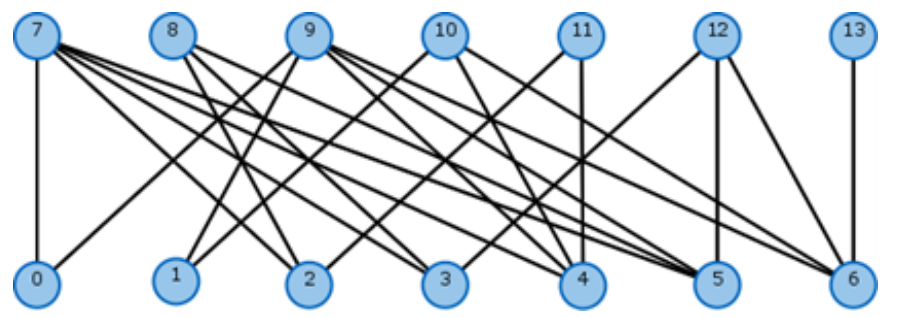
\includegraphics[scale=0.75]{graph_1.png}$$
\caption{graph\_1.png}
\end{figure}

    \textbf{Сочетанием (matching)} простого графа называется его
подмножество рёбер, никакие два из которых не имеют общей вершины.

\textbf{Задача о максимальном паросочетании (matching problem)}
заключается в нахождении по данному графу сочетания максимального
размера.

\textbf{Минимальное вершинное покрытие (minimum vertex cover, MVC)} ---
минимальный по размеру набор вершин, содержащий хотя бы один конец
каждого ребра.

\textbf{Мощность паросочетания} -- это количество рёбер в нём.

    Для решения задачи о максимальном паросочетании используется алгоритм
Форда-Фалкерсона. Суть алгоритма состоит в том, что вводятся две
фиктивные вершины истока и стока, и для обновленного графа применяется
алгоритм Форда-Фалкерсона для нахождения максимального потока в сети.

Знание максимального паросочетания позволяет получить минимальное
вершинное покрытие с помощью доказательства теоремы Кёнига -- в
произвольном двудольном графе мощность максимального паросочетания равна
мощности минимального вершинного покрытия. Это можно осуществить
следующим образом:

\begin{itemize}
\item
  При построенном паросочетанни, ориентируем ребра:
\item
  \begin{itemize}
  \tightlist
  \item
    Не из паросочетания -- из левой доли правую.
  \end{itemize}
\item
  \begin{itemize}
  \tightlist
  \item
    Из паросочетания -- из правой доли в левую.
  \end{itemize}
\item
  Запустить обход в глубину из всех свободных вершин левой доли и
  построить множества \(L^+,L^-,R^+,R^-\), где \(L^+,R^+\) -- вершины
  левой и правой доли, соответственно, посещенные обходом, а \(L^-,R^-\)
  -- вершины левой и правой доли, соответственно, не посещенные обходом.
\item
  В качестве результата взять \(L^-\cup R^+\).
\end{itemize}

    \begin{tcolorbox}[breakable, size=fbox, boxrule=1pt, pad at break*=1mm,colback=cellbackground, colframe=cellborder]
\prompt{In}{incolor}{2}{\boxspacing}
\begin{Verbatim}[commandchars=\\\{\}]
\PY{k}{def} \PY{n+nf}{find\PYZus{}max\PYZus{}matching}\PY{p}{(}\PY{n}{graph}\PY{p}{)}\PY{p}{:}
    \PY{n}{colors} \PY{o}{=} \PY{n}{split\PYZus{}graph}\PY{p}{(}\PY{n}{graph}\PY{p}{)}
    \PY{n}{net} \PY{o}{=} \PY{n}{build\PYZus{}net}\PY{p}{(}\PY{n}{graph}\PY{p}{,} \PY{n}{colors}\PY{p}{)}
    \PY{n}{matching} \PY{o}{=} \PY{p}{[}\PY{p}{]}
    \PY{k}{while} \PY{k+kc}{True}\PY{p}{:}
        \PY{n}{path} \PY{o}{=} \PY{n}{find\PYZus{}dfs\PYZus{}path}\PY{p}{(}\PY{n}{net}\PY{p}{,} \PY{l+s+s1}{\PYZsq{}}\PY{l+s+s1}{s}\PY{l+s+s1}{\PYZsq{}}\PY{p}{,} \PY{l+s+s1}{\PYZsq{}}\PY{l+s+s1}{t}\PY{l+s+s1}{\PYZsq{}}\PY{p}{)}
        \PY{k}{if} \PY{n}{path} \PY{o+ow}{is} \PY{k+kc}{None}\PY{p}{:}
            \PY{k}{break}
        \PY{n}{net}\PY{p}{[}\PY{l+s+s1}{\PYZsq{}}\PY{l+s+s1}{s}\PY{l+s+s1}{\PYZsq{}}\PY{p}{]}\PY{o}{.}\PY{n}{remove}\PY{p}{(}\PY{n}{path}\PY{p}{[}\PY{l+m+mi}{1}\PY{p}{]}\PY{p}{)}
        \PY{n}{net}\PY{p}{[}\PY{n}{path}\PY{p}{[}\PY{o}{\PYZhy{}}\PY{l+m+mi}{2}\PY{p}{]}\PY{p}{]}\PY{o}{.}\PY{n}{remove}\PY{p}{(}\PY{l+s+s1}{\PYZsq{}}\PY{l+s+s1}{t}\PY{l+s+s1}{\PYZsq{}}\PY{p}{)}
        \PY{k}{for} \PY{n}{i} \PY{o+ow}{in} \PY{n+nb}{range}\PY{p}{(}\PY{l+m+mi}{1}\PY{p}{,} \PY{n+nb}{len}\PY{p}{(}\PY{n}{path}\PY{p}{)} \PY{o}{\PYZhy{}} \PY{l+m+mi}{2}\PY{p}{)}\PY{p}{:}
            \PY{n}{net}\PY{p}{[}\PY{n}{path}\PY{p}{[}\PY{n}{i}\PY{p}{]}\PY{p}{]}\PY{o}{.}\PY{n}{remove}\PY{p}{(}\PY{n}{path}\PY{p}{[}\PY{n}{i} \PY{o}{+} \PY{l+m+mi}{1}\PY{p}{]}\PY{p}{)}
            \PY{n}{net}\PY{p}{[}\PY{n}{path}\PY{p}{[}\PY{n}{i} \PY{o}{+} \PY{l+m+mi}{1}\PY{p}{]}\PY{p}{]}\PY{o}{.}\PY{n}{append}\PY{p}{(}\PY{n}{path}\PY{p}{[}\PY{n}{i}\PY{p}{]}\PY{p}{)}
            \PY{n}{edge} \PY{o}{=} \PY{n+nb}{tuple}\PY{p}{(}\PY{n+nb}{sorted}\PY{p}{(}\PY{p}{[}\PY{n}{path}\PY{p}{[}\PY{n}{i}\PY{p}{]}\PY{p}{,} \PY{n}{path}\PY{p}{[}\PY{n}{i} \PY{o}{+} \PY{l+m+mi}{1}\PY{p}{]}\PY{p}{]}\PY{p}{)}\PY{p}{)}
            \PY{k}{if} \PY{n}{edge} \PY{o+ow}{in} \PY{n}{matching}\PY{p}{:}
                \PY{n}{matching}\PY{o}{.}\PY{n}{remove}\PY{p}{(}\PY{n}{edge}\PY{p}{)}
            \PY{k}{else}\PY{p}{:}
                \PY{n}{matching}\PY{o}{.}\PY{n}{append}\PY{p}{(}\PY{n}{edge}\PY{p}{)}
    \PY{k}{return} \PY{n}{matching}


\PY{k}{def} \PY{n+nf}{dfs}\PY{p}{(}\PY{n}{graph}\PY{p}{,} \PY{n}{start\PYZus{}node}\PY{p}{,} \PY{n}{visited}\PY{o}{=}\PY{k+kc}{None}\PY{p}{,} \PY{n}{from\PYZus{}}\PY{o}{=}\PY{k+kc}{None}\PY{p}{)}\PY{p}{:}
    \PY{k}{if} \PY{n}{visited} \PY{o+ow}{is} \PY{k+kc}{None}\PY{p}{:}
        \PY{n}{visited} \PY{o}{=} \PY{n+nb}{set}\PY{p}{(}\PY{p}{)}
    \PY{k}{if} \PY{n}{from\PYZus{}} \PY{o+ow}{is} \PY{k+kc}{None}\PY{p}{:}
        \PY{n}{from\PYZus{}} \PY{o}{=} \PY{p}{\PYZob{}}\PY{n}{key}\PY{p}{:} \PY{k+kc}{None} \PY{k}{for} \PY{n}{key} \PY{o+ow}{in} \PY{n}{graph}\PY{o}{.}\PY{n}{keys}\PY{p}{(}\PY{p}{)}\PY{p}{\PYZcb{}}
        \PY{n}{from\PYZus{}}\PY{p}{[}\PY{n}{start\PYZus{}node}\PY{p}{]} \PY{o}{=} \PY{n}{start\PYZus{}node}
    \PY{n}{visited}\PY{o}{.}\PY{n}{add}\PY{p}{(}\PY{n}{start\PYZus{}node}\PY{p}{)}
    \PY{k}{for} \PY{n}{neighbor} \PY{o+ow}{in} \PY{n}{graph}\PY{p}{[}\PY{n}{start\PYZus{}node}\PY{p}{]}\PY{p}{:}
        \PY{k}{if} \PY{n}{neighbor} \PY{o+ow}{not} \PY{o+ow}{in} \PY{n}{visited}\PY{p}{:}
            \PY{n}{from\PYZus{}}\PY{p}{[}\PY{n}{neighbor}\PY{p}{]} \PY{o}{=} \PY{n}{start\PYZus{}node}
            \PY{n}{dfs}\PY{p}{(}\PY{n}{graph}\PY{p}{,} \PY{n}{neighbor}\PY{p}{,} \PY{n}{visited}\PY{p}{,} \PY{n}{from\PYZus{}}\PY{p}{)}
    \PY{k}{return} \PY{n}{visited}\PY{p}{,} \PY{n}{from\PYZus{}}


\PY{k}{def} \PY{n+nf}{find\PYZus{}dfs\PYZus{}path}\PY{p}{(}\PY{n}{graph}\PY{p}{,} \PY{n}{start\PYZus{}node}\PY{p}{,} \PY{n}{end\PYZus{}node}\PY{p}{)}\PY{p}{:}
    \PY{n}{\PYZus{}}\PY{p}{,} \PY{n}{from\PYZus{}} \PY{o}{=} \PY{n}{dfs}\PY{p}{(}\PY{n}{graph}\PY{p}{,} \PY{n}{start\PYZus{}node}\PY{p}{)}
    \PY{n}{node} \PY{o}{=} \PY{n}{end\PYZus{}node}
    \PY{n}{path} \PY{o}{=} \PY{p}{[}\PY{p}{]}
    \PY{k}{while} \PY{k+kc}{True}\PY{p}{:}
        \PY{k}{if} \PY{n}{from\PYZus{}}\PY{p}{[}\PY{n}{node}\PY{p}{]} \PY{o+ow}{is} \PY{k+kc}{None}\PY{p}{:}
            \PY{k}{return} \PY{k+kc}{None}
        \PY{k}{if} \PY{n}{from\PYZus{}}\PY{p}{[}\PY{n}{node}\PY{p}{]} \PY{o}{!=} \PY{n}{node}\PY{p}{:}
            \PY{n}{path}\PY{o}{.}\PY{n}{append}\PY{p}{(}\PY{n}{node}\PY{p}{)}
            \PY{n}{node} \PY{o}{=} \PY{n}{from\PYZus{}}\PY{p}{[}\PY{n}{node}\PY{p}{]}
        \PY{k}{else}\PY{p}{:}
            \PY{k}{break}
    \PY{n}{path}\PY{o}{.}\PY{n}{append}\PY{p}{(}\PY{n}{start\PYZus{}node}\PY{p}{)}
    \PY{k}{return} \PY{n+nb}{list}\PY{p}{(}\PY{n+nb}{reversed}\PY{p}{(}\PY{n}{path}\PY{p}{)}\PY{p}{)}


\PY{k}{def} \PY{n+nf}{split\PYZus{}graph}\PY{p}{(}\PY{n}{graph}\PY{p}{)}\PY{p}{:}
    \PY{n}{colors} \PY{o}{=} \PY{p}{\PYZob{}}\PY{n}{key}\PY{p}{:} \PY{k+kc}{None} \PY{k}{for} \PY{n}{key} \PY{o+ow}{in} \PY{n}{graph}\PY{o}{.}\PY{n}{keys}\PY{p}{(}\PY{p}{)}\PY{p}{\PYZcb{}}

    \PY{k}{def} \PY{n+nf}{set\PYZus{}color}\PY{p}{(}\PY{n}{node}\PY{p}{)}\PY{p}{:}
        \PY{n}{cur\PYZus{}color} \PY{o}{=} \PY{n}{colors}\PY{p}{[}\PY{n}{node}\PY{p}{]}
        \PY{n}{neighbor\PYZus{}color} \PY{o}{=} \PY{l+s+s1}{\PYZsq{}}\PY{l+s+s1}{r}\PY{l+s+s1}{\PYZsq{}} \PY{k}{if} \PY{n}{cur\PYZus{}color} \PY{o}{==} \PY{l+s+s1}{\PYZsq{}}\PY{l+s+s1}{l}\PY{l+s+s1}{\PYZsq{}} \PY{k}{else} \PY{l+s+s1}{\PYZsq{}}\PY{l+s+s1}{l}\PY{l+s+s1}{\PYZsq{}}
        \PY{k}{for} \PY{n}{g} \PY{o+ow}{in} \PY{n}{graph}\PY{p}{[}\PY{n}{node}\PY{p}{]}\PY{p}{:}
            \PY{k}{if} \PY{n}{colors}\PY{p}{[}\PY{n}{g}\PY{p}{]} \PY{o+ow}{is} \PY{k+kc}{None}\PY{p}{:}
                \PY{n}{colors}\PY{p}{[}\PY{n}{g}\PY{p}{]} \PY{o}{=} \PY{n}{neighbor\PYZus{}color}
                \PY{n}{set\PYZus{}color}\PY{p}{(}\PY{n}{g}\PY{p}{)}

    \PY{k}{for} \PY{n}{node} \PY{o+ow}{in} \PY{n}{graph}\PY{o}{.}\PY{n}{keys}\PY{p}{(}\PY{p}{)}\PY{p}{:}
        \PY{k}{if} \PY{n}{colors}\PY{p}{[}\PY{n}{node}\PY{p}{]} \PY{o+ow}{is} \PY{k+kc}{None}\PY{p}{:}
            \PY{n}{colors}\PY{p}{[}\PY{n}{node}\PY{p}{]} \PY{o}{=} \PY{l+s+s1}{\PYZsq{}}\PY{l+s+s1}{l}\PY{l+s+s1}{\PYZsq{}}
            \PY{n}{set\PYZus{}color}\PY{p}{(}\PY{n}{node}\PY{p}{)}
    \PY{n}{res} \PY{o}{=} \PY{p}{\PYZob{}}\PY{l+s+s1}{\PYZsq{}}\PY{l+s+s1}{l}\PY{l+s+s1}{\PYZsq{}}\PY{p}{:} \PY{p}{[}\PY{p}{]}\PY{p}{,} \PY{l+s+s1}{\PYZsq{}}\PY{l+s+s1}{r}\PY{l+s+s1}{\PYZsq{}}\PY{p}{:} \PY{p}{[}\PY{p}{]}\PY{p}{\PYZcb{}}
    \PY{k}{for} \PY{n}{key}\PY{p}{,} \PY{n}{value} \PY{o+ow}{in} \PY{n}{colors}\PY{o}{.}\PY{n}{items}\PY{p}{(}\PY{p}{)}\PY{p}{:}
        \PY{k}{if} \PY{n}{value} \PY{o}{==} \PY{l+s+s1}{\PYZsq{}}\PY{l+s+s1}{l}\PY{l+s+s1}{\PYZsq{}}\PY{p}{:}
            \PY{n}{res}\PY{p}{[}\PY{l+s+s1}{\PYZsq{}}\PY{l+s+s1}{l}\PY{l+s+s1}{\PYZsq{}}\PY{p}{]}\PY{o}{.}\PY{n}{append}\PY{p}{(}\PY{n}{key}\PY{p}{)}
        \PY{k}{else}\PY{p}{:}
            \PY{n}{res}\PY{p}{[}\PY{l+s+s1}{\PYZsq{}}\PY{l+s+s1}{r}\PY{l+s+s1}{\PYZsq{}}\PY{p}{]}\PY{o}{.}\PY{n}{append}\PY{p}{(}\PY{n}{key}\PY{p}{)}
    \PY{k}{return} \PY{n}{res}


\PY{k}{def} \PY{n+nf}{build\PYZus{}net}\PY{p}{(}\PY{n}{graph}\PY{p}{,} \PY{n}{colors}\PY{p}{)}\PY{p}{:}
    \PY{n}{net} \PY{o}{=} \PY{p}{\PYZob{}}\PY{n}{key}\PY{p}{:} \PY{p}{[}\PY{p}{]} \PY{k}{for} \PY{n}{key} \PY{o+ow}{in} \PY{n}{graph}\PY{o}{.}\PY{n}{keys}\PY{p}{(}\PY{p}{)}\PY{p}{\PYZcb{}}
    \PY{n}{net}\PY{p}{[}\PY{l+s+s1}{\PYZsq{}}\PY{l+s+s1}{s}\PY{l+s+s1}{\PYZsq{}}\PY{p}{]} \PY{o}{=} \PY{n}{colors}\PY{p}{[}\PY{l+s+s1}{\PYZsq{}}\PY{l+s+s1}{l}\PY{l+s+s1}{\PYZsq{}}\PY{p}{]}
    \PY{n}{net}\PY{p}{[}\PY{l+s+s1}{\PYZsq{}}\PY{l+s+s1}{t}\PY{l+s+s1}{\PYZsq{}}\PY{p}{]} \PY{o}{=} \PY{p}{[}\PY{p}{]}
    \PY{k}{for} \PY{n}{u} \PY{o+ow}{in} \PY{n}{colors}\PY{p}{[}\PY{l+s+s1}{\PYZsq{}}\PY{l+s+s1}{r}\PY{l+s+s1}{\PYZsq{}}\PY{p}{]}\PY{p}{:}
        \PY{n}{net}\PY{p}{[}\PY{n}{u}\PY{p}{]}\PY{o}{.}\PY{n}{append}\PY{p}{(}\PY{l+s+s1}{\PYZsq{}}\PY{l+s+s1}{t}\PY{l+s+s1}{\PYZsq{}}\PY{p}{)}
    \PY{k}{for} \PY{n}{u} \PY{o+ow}{in} \PY{n}{colors}\PY{p}{[}\PY{l+s+s1}{\PYZsq{}}\PY{l+s+s1}{l}\PY{l+s+s1}{\PYZsq{}}\PY{p}{]}\PY{p}{:}
        \PY{k}{for} \PY{n}{v} \PY{o+ow}{in} \PY{n}{graph}\PY{p}{[}\PY{n}{u}\PY{p}{]}\PY{p}{:}
            \PY{n}{net}\PY{p}{[}\PY{n}{u}\PY{p}{]}\PY{o}{.}\PY{n}{append}\PY{p}{(}\PY{n}{v}\PY{p}{)}
    \PY{k}{return} \PY{n}{net}


\PY{k}{def} \PY{n+nf}{find\PYZus{}min\PYZus{}coverage}\PY{p}{(}\PY{n}{graph}\PY{p}{,} \PY{n}{max\PYZus{}matching}\PY{p}{)}\PY{p}{:}
    \PY{n}{colors} \PY{o}{=} \PY{n}{split\PYZus{}graph}\PY{p}{(}\PY{n}{graph}\PY{p}{)}
    \PY{n}{help\PYZus{}graph} \PY{o}{=} \PY{n}{build\PYZus{}help\PYZus{}graph}\PY{p}{(}\PY{n}{graph}\PY{p}{,} \PY{n}{colors}\PY{p}{,} \PY{n}{max\PYZus{}matching}\PY{p}{)}
    \PY{n}{L} \PY{o}{=} \PY{n+nb}{set}\PY{p}{(}\PY{n}{colors}\PY{p}{[}\PY{l+s+s1}{\PYZsq{}}\PY{l+s+s1}{l}\PY{l+s+s1}{\PYZsq{}}\PY{p}{]}\PY{p}{)}
    \PY{n}{R} \PY{o}{=} \PY{n+nb}{set}\PY{p}{(}\PY{n}{colors}\PY{p}{[}\PY{l+s+s1}{\PYZsq{}}\PY{l+s+s1}{r}\PY{l+s+s1}{\PYZsq{}}\PY{p}{]}\PY{p}{)}
    \PY{n}{match\PYZus{}set} \PY{o}{=} \PY{n+nb}{set}\PY{p}{(}\PY{p}{)}
    \PY{k}{for} \PY{n}{edge} \PY{o+ow}{in} \PY{n}{max\PYZus{}matching}\PY{p}{:}
        \PY{n}{match\PYZus{}set}\PY{o}{.}\PY{n}{add}\PY{p}{(}\PY{n}{edge}\PY{p}{[}\PY{l+m+mi}{0}\PY{p}{]}\PY{p}{)}
        \PY{n}{match\PYZus{}set}\PY{o}{.}\PY{n}{add}\PY{p}{(}\PY{n}{edge}\PY{p}{[}\PY{l+m+mi}{1}\PY{p}{]}\PY{p}{)}
    \PY{n}{visited} \PY{o}{=} \PY{n+nb}{set}\PY{p}{(}\PY{p}{)}
    \PY{k}{for} \PY{n}{v} \PY{o+ow}{in} \PY{p}{(}\PY{n}{L} \PY{o}{\PYZhy{}} \PY{n}{match\PYZus{}set}\PY{p}{)}\PY{p}{:}
        \PY{n}{vis}\PY{p}{,} \PY{n}{\PYZus{}} \PY{o}{=} \PY{n}{dfs}\PY{p}{(}\PY{n}{help\PYZus{}graph}\PY{p}{,} \PY{n}{v}\PY{p}{,} \PY{n}{visited}\PY{o}{=}\PY{n}{visited}\PY{p}{)}
        \PY{n}{visited} \PY{o}{=} \PY{n}{vis} \PY{o}{|} \PY{n}{visited}
    \PY{k}{return} \PY{n+nb}{list}\PY{p}{(}\PY{p}{(}\PY{n}{L} \PY{o}{\PYZhy{}} \PY{n}{visited}\PY{p}{)} \PY{o}{|} \PY{p}{(}\PY{n}{R} \PY{o}{\PYZam{}} \PY{n}{visited}\PY{p}{)}\PY{p}{)}


\PY{k}{def} \PY{n+nf}{build\PYZus{}help\PYZus{}graph}\PY{p}{(}\PY{n}{graph}\PY{p}{,} \PY{n}{colors}\PY{p}{,} \PY{n}{max\PYZus{}matching}\PY{p}{)}\PY{p}{:}
    \PY{n}{new\PYZus{}graph} \PY{o}{=} \PY{p}{\PYZob{}}\PY{n}{key}\PY{p}{:} \PY{p}{[}\PY{p}{]} \PY{k}{for} \PY{n}{key} \PY{o+ow}{in} \PY{n}{graph}\PY{o}{.}\PY{n}{keys}\PY{p}{(}\PY{p}{)}\PY{p}{\PYZcb{}}
    \PY{n}{edges} \PY{o}{=} \PY{n}{get\PYZus{}all\PYZus{}edges\PYZus{}of\PYZus{}bipartite\PYZus{}graph}\PY{p}{(}\PY{n}{graph}\PY{p}{,} \PY{n}{colors}\PY{p}{)}
    \PY{k}{for} \PY{n}{edge} \PY{o+ow}{in} \PY{n}{edges}\PY{p}{:}
        \PY{n}{start} \PY{o}{=} \PY{n}{edge}\PY{p}{[}\PY{l+m+mi}{0}\PY{p}{]}
        \PY{n}{end} \PY{o}{=} \PY{n}{edge}\PY{p}{[}\PY{l+m+mi}{1}\PY{p}{]}
        \PY{k}{if} \PY{n}{edge} \PY{o+ow}{in} \PY{n}{max\PYZus{}matching}\PY{p}{:}
            \PY{k}{if} \PY{n}{start} \PY{o+ow}{in} \PY{n}{colors}\PY{p}{[}\PY{l+s+s1}{\PYZsq{}}\PY{l+s+s1}{l}\PY{l+s+s1}{\PYZsq{}}\PY{p}{]}\PY{p}{:}
                \PY{n}{new\PYZus{}graph}\PY{p}{[}\PY{n}{end}\PY{p}{]}\PY{o}{.}\PY{n}{append}\PY{p}{(}\PY{n}{start}\PY{p}{)}
            \PY{k}{else}\PY{p}{:}
                \PY{n}{new\PYZus{}graph}\PY{p}{[}\PY{n}{start}\PY{p}{]}\PY{o}{.}\PY{n}{append}\PY{p}{(}\PY{n}{end}\PY{p}{)}
        \PY{k}{else}\PY{p}{:}
            \PY{k}{if} \PY{n}{start} \PY{o+ow}{in} \PY{n}{colors}\PY{p}{[}\PY{l+s+s1}{\PYZsq{}}\PY{l+s+s1}{l}\PY{l+s+s1}{\PYZsq{}}\PY{p}{]}\PY{p}{:}
                \PY{n}{new\PYZus{}graph}\PY{p}{[}\PY{n}{start}\PY{p}{]}\PY{o}{.}\PY{n}{append}\PY{p}{(}\PY{n}{end}\PY{p}{)}
            \PY{k}{else}\PY{p}{:}
                \PY{n}{new\PYZus{}graph}\PY{p}{[}\PY{n}{end}\PY{p}{]}\PY{o}{.}\PY{n}{append}\PY{p}{(}\PY{n}{start}\PY{p}{)}
    \PY{k}{return} \PY{n}{new\PYZus{}graph}


\PY{k}{def} \PY{n+nf}{get\PYZus{}all\PYZus{}edges\PYZus{}of\PYZus{}bipartite\PYZus{}graph}\PY{p}{(}\PY{n}{graph}\PY{p}{,} \PY{n}{colors}\PY{p}{)}\PY{p}{:}
    \PY{n}{edges} \PY{o}{=} \PY{p}{[}\PY{p}{]}
    \PY{k}{for} \PY{n}{u} \PY{o+ow}{in} \PY{n}{colors}\PY{p}{[}\PY{l+s+s1}{\PYZsq{}}\PY{l+s+s1}{l}\PY{l+s+s1}{\PYZsq{}}\PY{p}{]}\PY{p}{:}
        \PY{k}{for} \PY{n}{v} \PY{o+ow}{in} \PY{n}{graph}\PY{p}{[}\PY{n}{u}\PY{p}{]}\PY{p}{:}
            \PY{n}{edges}\PY{o}{.}\PY{n}{append}\PY{p}{(}\PY{n+nb}{tuple}\PY{p}{(}\PY{n+nb}{sorted}\PY{p}{(}\PY{p}{[}\PY{n}{u}\PY{p}{,} \PY{n}{v}\PY{p}{]}\PY{p}{)}\PY{p}{)}\PY{p}{)}
    \PY{k}{return} \PY{n}{edges}

\PY{n}{graph} \PY{o}{=} \PY{p}{\PYZob{}}
 \PY{l+m+mi}{0}\PY{p}{:} \PY{p}{[}\PY{l+m+mi}{6}\PY{p}{]}\PY{p}{,}
 \PY{l+m+mi}{1}\PY{p}{:} \PY{p}{[}\PY{l+m+mi}{6}\PY{p}{,} \PY{l+m+mi}{7}\PY{p}{,} \PY{l+m+mi}{9}\PY{p}{]}\PY{p}{,}
 \PY{l+m+mi}{2}\PY{p}{:} \PY{p}{[}\PY{l+m+mi}{7}\PY{p}{,} \PY{l+m+mi}{8}\PY{p}{,} \PY{l+m+mi}{10}\PY{p}{]}\PY{p}{,}
 \PY{l+m+mi}{3}\PY{p}{:} \PY{p}{[}\PY{l+m+mi}{7}\PY{p}{,} \PY{l+m+mi}{8}\PY{p}{,} \PY{l+m+mi}{9}\PY{p}{]}\PY{p}{,}
 \PY{l+m+mi}{4}\PY{p}{:} \PY{p}{[}\PY{l+m+mi}{10}\PY{p}{,} \PY{l+m+mi}{11}\PY{p}{]}\PY{p}{,}
 \PY{l+m+mi}{5}\PY{p}{:} \PY{p}{[}\PY{l+m+mi}{6}\PY{p}{,} \PY{l+m+mi}{9}\PY{p}{]}\PY{p}{,}
 \PY{l+m+mi}{6}\PY{p}{:} \PY{p}{[}\PY{l+m+mi}{0}\PY{p}{,} \PY{l+m+mi}{1}\PY{p}{,} \PY{l+m+mi}{5}\PY{p}{]}\PY{p}{,}
 \PY{l+m+mi}{7}\PY{p}{:} \PY{p}{[}\PY{l+m+mi}{1}\PY{p}{,} \PY{l+m+mi}{2}\PY{p}{,} \PY{l+m+mi}{3}\PY{p}{]}\PY{p}{,}
 \PY{l+m+mi}{8}\PY{p}{:} \PY{p}{[}\PY{l+m+mi}{2}\PY{p}{,} \PY{l+m+mi}{3}\PY{p}{]}\PY{p}{,}
 \PY{l+m+mi}{9}\PY{p}{:} \PY{p}{[}\PY{l+m+mi}{1}\PY{p}{,} \PY{l+m+mi}{3}\PY{p}{,} \PY{l+m+mi}{5}\PY{p}{]}\PY{p}{,}
 \PY{l+m+mi}{10}\PY{p}{:} \PY{p}{[}\PY{l+m+mi}{2}\PY{p}{,} \PY{l+m+mi}{4}\PY{p}{]}\PY{p}{,}
 \PY{l+m+mi}{11}\PY{p}{:} \PY{p}{[}\PY{l+m+mi}{4}\PY{p}{,} \PY{p}{]}\PY{p}{,}
\PY{p}{\PYZcb{}}

\PY{n}{graph1} \PY{o}{=} \PY{p}{\PYZob{}}
    \PY{l+m+mi}{0}\PY{p}{:} \PY{p}{[}\PY{l+m+mi}{7}\PY{p}{,} \PY{l+m+mi}{9}\PY{p}{]}\PY{p}{,}
    \PY{l+m+mi}{1}\PY{p}{:} \PY{p}{[}\PY{l+m+mi}{9}\PY{p}{,} \PY{l+m+mi}{10}\PY{p}{]}\PY{p}{,}
    \PY{l+m+mi}{2}\PY{p}{:} \PY{p}{[}\PY{l+m+mi}{7}\PY{p}{,} \PY{l+m+mi}{11}\PY{p}{]}\PY{p}{,}
    \PY{l+m+mi}{3}\PY{p}{:} \PY{p}{[}\PY{l+m+mi}{7}\PY{p}{,} \PY{l+m+mi}{8}\PY{p}{,} \PY{l+m+mi}{12}\PY{p}{]}\PY{p}{,}
    \PY{l+m+mi}{4}\PY{p}{:} \PY{p}{[}\PY{l+m+mi}{7}\PY{p}{,} \PY{l+m+mi}{9}\PY{p}{,} \PY{l+m+mi}{10}\PY{p}{,} \PY{l+m+mi}{11}\PY{p}{]}\PY{p}{,}
    \PY{l+m+mi}{5}\PY{p}{:} \PY{p}{[}\PY{l+m+mi}{7}\PY{p}{,} \PY{l+m+mi}{8}\PY{p}{,} \PY{l+m+mi}{9}\PY{p}{,} \PY{l+m+mi}{12}\PY{p}{]}\PY{p}{,}
    \PY{l+m+mi}{6}\PY{p}{:} \PY{p}{[}\PY{l+m+mi}{9}\PY{p}{,} \PY{l+m+mi}{10}\PY{p}{,} \PY{l+m+mi}{13}\PY{p}{]}\PY{p}{,}
    \PY{l+m+mi}{7}\PY{p}{:} \PY{p}{[}\PY{l+m+mi}{2}\PY{p}{,} \PY{l+m+mi}{3}\PY{p}{,} \PY{l+m+mi}{4}\PY{p}{,} \PY{l+m+mi}{5}\PY{p}{]}\PY{p}{,}
    \PY{l+m+mi}{8}\PY{p}{:} \PY{p}{[}\PY{l+m+mi}{2}\PY{p}{,} \PY{l+m+mi}{3}\PY{p}{,} \PY{l+m+mi}{5}\PY{p}{]}\PY{p}{,}
    \PY{l+m+mi}{9}\PY{p}{:} \PY{p}{[}\PY{l+m+mi}{0}\PY{p}{,} \PY{l+m+mi}{1}\PY{p}{,} \PY{l+m+mi}{4}\PY{p}{,} \PY{l+m+mi}{5}\PY{p}{,} \PY{l+m+mi}{6}\PY{p}{]}\PY{p}{,}
    \PY{l+m+mi}{10}\PY{p}{:} \PY{p}{[}\PY{l+m+mi}{1}\PY{p}{,} \PY{l+m+mi}{4}\PY{p}{,} \PY{l+m+mi}{6}\PY{p}{]}\PY{p}{,}
    \PY{l+m+mi}{11}\PY{p}{:} \PY{p}{[}\PY{l+m+mi}{2}\PY{p}{,} \PY{l+m+mi}{4}\PY{p}{]}\PY{p}{,}
    \PY{l+m+mi}{12}\PY{p}{:} \PY{p}{[}\PY{l+m+mi}{3}\PY{p}{,} \PY{l+m+mi}{5}\PY{p}{,} \PY{l+m+mi}{6}\PY{p}{]}\PY{p}{,}
    \PY{l+m+mi}{13}\PY{p}{:} \PY{p}{[}\PY{l+m+mi}{6}\PY{p}{]}
\PY{p}{\PYZcb{}}

\PY{n}{max\PYZus{}matching} \PY{o}{=} \PY{n}{find\PYZus{}max\PYZus{}matching}\PY{p}{(}\PY{n}{graph}\PY{p}{)}
\PY{n}{min\PYZus{}coverage} \PY{o}{=} \PY{n}{find\PYZus{}min\PYZus{}coverage}\PY{p}{(}\PY{n}{graph}\PY{p}{,} \PY{n}{max\PYZus{}matching}\PY{p}{)}
\PY{n+nb}{print}\PY{p}{(}\PY{l+s+sa}{f}\PY{l+s+s1}{\PYZsq{}}\PY{l+s+s1}{Максимальное паросочетание: }\PY{l+s+si}{\PYZob{}}\PY{n}{max\PYZus{}matching}\PY{l+s+si}{\PYZcb{}}\PY{l+s+s1}{\PYZsq{}}\PY{p}{)}
\PY{n+nb}{print}\PY{p}{(}\PY{l+s+sa}{f}\PY{l+s+s1}{\PYZsq{}}\PY{l+s+s1}{Минимальное покрытие: }\PY{l+s+si}{\PYZob{}}\PY{n}{min\PYZus{}coverage}\PY{l+s+si}{\PYZcb{}}\PY{l+s+s1}{\PYZsq{}}\PY{p}{)}
\end{Verbatim}
\end{tcolorbox}

    \begin{Verbatim}[commandchars=\\\{\}]
Максимальное паросочетание: [(0, 6), (5, 9), (1, 7), (3, 8), (2, 10), (4, 11)]
Минимальное покрытие: [0, 1, 2, 3, 4, 5]
    \end{Verbatim}

    \section{Задача о
назначениях}\label{ux437ux430ux434ux430ux447ux430-ux43e-ux43dux430ux437ux43dux430ux447ux435ux43dux438ux44fux445}

    Решите задачу о назначениях:

\begin{table}[h]
\centering
\begin{tabular}{|c|c|c|c|c|}
\hline
2 & 4 & 1 & 4 & 2 \\
\hline
1 & 3 & 2 & 2 & 4 \\
\hline
3 & 2 & 5 & 2 & 3 \\
\hline
1 & 3 & 2 & 5 & 2 \\
\hline
2 & 1 & 3 & 3 & 2\\
\hline
\end{tabular}
\end{table}

\textbf{Постановка задачи о назначениях.} Для \(n\) работников и работ,
дана матрица \(n \times n\), задающая стоимость выполнения каждой работы
каждым работником. Найти минимальную стоимость выполнения работ, такую
что каждый работник выполняет ровно одну работу, а каждую работу
выполняет ровно один работник. Т.е. произвести назначение (assignment)
работника на работу.

Назначение можно задать биекцией между двумя конечными множествами из
\(n\) элементов, которая задается перестановкой
\((p_1, p_2,\dots, p_n)\).

Решать задачу будет компьютерными методам с помощью библиотеки OR-Tools.

    \begin{tcolorbox}[breakable, size=fbox, boxrule=1pt, pad at break*=1mm,colback=cellbackground, colframe=cellborder]
\prompt{In}{incolor}{2}{\boxspacing}
\begin{Verbatim}[commandchars=\\\{\}]
\PY{c+c1}{\PYZsh{}pip install ortools}
\end{Verbatim}
\end{tcolorbox}

    \begin{tcolorbox}[breakable, size=fbox, boxrule=1pt, pad at break*=1mm,colback=cellbackground, colframe=cellborder]
\prompt{In}{incolor}{7}{\boxspacing}
\begin{Verbatim}[commandchars=\\\{\}]
\PY{k+kn}{from} \PY{n+nn}{ortools}\PY{n+nn}{.}\PY{n+nn}{linear\PYZus{}solver} \PY{k+kn}{import} \PY{n}{pywraplp}


\PY{k}{def} \PY{n+nf}{assignment\PYZus{}problem}\PY{p}{(}\PY{p}{)}\PY{p}{:}
    \PY{c+c1}{\PYZsh{} Data}
    \PY{n}{costs} \PY{o}{=} \PY{p}{[}
        \PY{p}{[}\PY{l+m+mi}{2}\PY{p}{,} \PY{l+m+mi}{4}\PY{p}{,} \PY{l+m+mi}{1}\PY{p}{,} \PY{l+m+mi}{4}\PY{p}{,} \PY{l+m+mi}{2}\PY{p}{]}\PY{p}{,}
        \PY{p}{[}\PY{l+m+mi}{1}\PY{p}{,} \PY{l+m+mi}{3}\PY{p}{,} \PY{l+m+mi}{2}\PY{p}{,} \PY{l+m+mi}{2}\PY{p}{,} \PY{l+m+mi}{4}\PY{p}{]}\PY{p}{,}
        \PY{p}{[}\PY{l+m+mi}{3}\PY{p}{,} \PY{l+m+mi}{2}\PY{p}{,} \PY{l+m+mi}{5}\PY{p}{,} \PY{l+m+mi}{2}\PY{p}{,} \PY{l+m+mi}{3}\PY{p}{]}\PY{p}{,}
        \PY{p}{[}\PY{l+m+mi}{1}\PY{p}{,} \PY{l+m+mi}{3}\PY{p}{,} \PY{l+m+mi}{2}\PY{p}{,} \PY{l+m+mi}{5}\PY{p}{,} \PY{l+m+mi}{2}\PY{p}{]}\PY{p}{,}
        \PY{p}{[}\PY{l+m+mi}{2}\PY{p}{,} \PY{l+m+mi}{1}\PY{p}{,} \PY{l+m+mi}{3}\PY{p}{,} \PY{l+m+mi}{3}\PY{p}{,} \PY{l+m+mi}{2}\PY{p}{]}\PY{p}{,}
    \PY{p}{]}
    
    \PY{n}{num\PYZus{}workers} \PY{o}{=} \PY{n+nb}{len}\PY{p}{(}\PY{n}{costs}\PY{p}{)}
    \PY{n}{num\PYZus{}tasks} \PY{o}{=} \PY{n+nb}{len}\PY{p}{(}\PY{n}{costs}\PY{p}{[}\PY{l+m+mi}{0}\PY{p}{]}\PY{p}{)}

    \PY{c+c1}{\PYZsh{} Solver}
    \PY{c+c1}{\PYZsh{} Create the mip solver with the SCIP backend.}
    \PY{n}{solver} \PY{o}{=} \PY{n}{pywraplp}\PY{o}{.}\PY{n}{Solver}\PY{o}{.}\PY{n}{CreateSolver}\PY{p}{(}\PY{l+s+s2}{\PYZdq{}}\PY{l+s+s2}{SCIP}\PY{l+s+s2}{\PYZdq{}}\PY{p}{)}

    \PY{k}{if} \PY{o+ow}{not} \PY{n}{solver}\PY{p}{:}
        \PY{k}{return}

    \PY{c+c1}{\PYZsh{} Variables}
    \PY{c+c1}{\PYZsh{} x[i, j] is an array of 0\PYZhy{}1 variables, which will be 1}
    \PY{c+c1}{\PYZsh{} if worker i is assigned to task j.}
    \PY{n}{x} \PY{o}{=} \PY{p}{\PYZob{}}\PY{p}{\PYZcb{}}
    \PY{k}{for} \PY{n}{i} \PY{o+ow}{in} \PY{n+nb}{range}\PY{p}{(}\PY{n}{num\PYZus{}workers}\PY{p}{)}\PY{p}{:}
        \PY{k}{for} \PY{n}{j} \PY{o+ow}{in} \PY{n+nb}{range}\PY{p}{(}\PY{n}{num\PYZus{}tasks}\PY{p}{)}\PY{p}{:}
            \PY{n}{x}\PY{p}{[}\PY{n}{i}\PY{p}{,} \PY{n}{j}\PY{p}{]} \PY{o}{=} \PY{n}{solver}\PY{o}{.}\PY{n}{IntVar}\PY{p}{(}\PY{l+m+mi}{0}\PY{p}{,} \PY{l+m+mi}{1}\PY{p}{,} \PY{l+s+s2}{\PYZdq{}}\PY{l+s+s2}{\PYZdq{}}\PY{p}{)}

    \PY{c+c1}{\PYZsh{} Constraints}
    \PY{c+c1}{\PYZsh{} Each worker is assigned to at most 1 task.}
    \PY{k}{for} \PY{n}{i} \PY{o+ow}{in} \PY{n+nb}{range}\PY{p}{(}\PY{n}{num\PYZus{}workers}\PY{p}{)}\PY{p}{:}
        \PY{n}{solver}\PY{o}{.}\PY{n}{Add}\PY{p}{(}\PY{n}{solver}\PY{o}{.}\PY{n}{Sum}\PY{p}{(}\PY{p}{[}\PY{n}{x}\PY{p}{[}\PY{n}{i}\PY{p}{,} \PY{n}{j}\PY{p}{]} \PY{k}{for} \PY{n}{j} \PY{o+ow}{in} \PY{n+nb}{range}\PY{p}{(}\PY{n}{num\PYZus{}tasks}\PY{p}{)}\PY{p}{]}\PY{p}{)} \PY{o}{\PYZlt{}}\PY{o}{=} \PY{l+m+mi}{1}\PY{p}{)}

    \PY{c+c1}{\PYZsh{} Each task is assigned to exactly one worker.}
    \PY{k}{for} \PY{n}{j} \PY{o+ow}{in} \PY{n+nb}{range}\PY{p}{(}\PY{n}{num\PYZus{}tasks}\PY{p}{)}\PY{p}{:}
        \PY{n}{solver}\PY{o}{.}\PY{n}{Add}\PY{p}{(}\PY{n}{solver}\PY{o}{.}\PY{n}{Sum}\PY{p}{(}\PY{p}{[}\PY{n}{x}\PY{p}{[}\PY{n}{i}\PY{p}{,} \PY{n}{j}\PY{p}{]} \PY{k}{for} \PY{n}{i} \PY{o+ow}{in} \PY{n+nb}{range}\PY{p}{(}\PY{n}{num\PYZus{}workers}\PY{p}{)}\PY{p}{]}\PY{p}{)} \PY{o}{==} \PY{l+m+mi}{1}\PY{p}{)}

    \PY{c+c1}{\PYZsh{} Objective}
    \PY{n}{objective\PYZus{}terms} \PY{o}{=} \PY{p}{[}\PY{p}{]}
    \PY{k}{for} \PY{n}{i} \PY{o+ow}{in} \PY{n+nb}{range}\PY{p}{(}\PY{n}{num\PYZus{}workers}\PY{p}{)}\PY{p}{:}
        \PY{k}{for} \PY{n}{j} \PY{o+ow}{in} \PY{n+nb}{range}\PY{p}{(}\PY{n}{num\PYZus{}tasks}\PY{p}{)}\PY{p}{:}
            \PY{n}{objective\PYZus{}terms}\PY{o}{.}\PY{n}{append}\PY{p}{(}\PY{n}{costs}\PY{p}{[}\PY{n}{i}\PY{p}{]}\PY{p}{[}\PY{n}{j}\PY{p}{]} \PY{o}{*} \PY{n}{x}\PY{p}{[}\PY{n}{i}\PY{p}{,} \PY{n}{j}\PY{p}{]}\PY{p}{)}
    \PY{n}{solver}\PY{o}{.}\PY{n}{Minimize}\PY{p}{(}\PY{n}{solver}\PY{o}{.}\PY{n}{Sum}\PY{p}{(}\PY{n}{objective\PYZus{}terms}\PY{p}{)}\PY{p}{)}

    \PY{c+c1}{\PYZsh{} Solve}
    \PY{n+nb}{print}\PY{p}{(}\PY{l+s+sa}{f}\PY{l+s+s2}{\PYZdq{}}\PY{l+s+s2}{Solving with }\PY{l+s+si}{\PYZob{}}\PY{n}{solver}\PY{o}{.}\PY{n}{SolverVersion}\PY{p}{(}\PY{p}{)}\PY{l+s+si}{\PYZcb{}}\PY{l+s+s2}{\PYZdq{}}\PY{p}{)}
    \PY{n}{status} \PY{o}{=} \PY{n}{solver}\PY{o}{.}\PY{n}{Solve}\PY{p}{(}\PY{p}{)}

    \PY{c+c1}{\PYZsh{} Print solution.}
    \PY{k}{if} \PY{n}{status} \PY{o}{==} \PY{n}{pywraplp}\PY{o}{.}\PY{n}{Solver}\PY{o}{.}\PY{n}{OPTIMAL} \PY{o+ow}{or} \PY{n}{status} \PY{o}{==} \PY{n}{pywraplp}\PY{o}{.}\PY{n}{Solver}\PY{o}{.}\PY{n}{FEASIBLE}\PY{p}{:}
        \PY{n+nb}{print}\PY{p}{(}\PY{l+s+sa}{f}\PY{l+s+s2}{\PYZdq{}}\PY{l+s+s2}{Total cost = }\PY{l+s+si}{\PYZob{}}\PY{n}{solver}\PY{o}{.}\PY{n}{Objective}\PY{p}{(}\PY{p}{)}\PY{o}{.}\PY{n}{Value}\PY{p}{(}\PY{p}{)}\PY{l+s+si}{\PYZcb{}}\PY{l+s+se}{\PYZbs{}n}\PY{l+s+s2}{\PYZdq{}}\PY{p}{)}
        \PY{k}{for} \PY{n}{i} \PY{o+ow}{in} \PY{n+nb}{range}\PY{p}{(}\PY{n}{num\PYZus{}workers}\PY{p}{)}\PY{p}{:}
            \PY{k}{for} \PY{n}{j} \PY{o+ow}{in} \PY{n+nb}{range}\PY{p}{(}\PY{n}{num\PYZus{}tasks}\PY{p}{)}\PY{p}{:}
                \PY{c+c1}{\PYZsh{} Test if x[i,j] is 1 (with tolerance for floating point arithmetic).}
                \PY{k}{if} \PY{n}{x}\PY{p}{[}\PY{n}{i}\PY{p}{,} \PY{n}{j}\PY{p}{]}\PY{o}{.}\PY{n}{solution\PYZus{}value}\PY{p}{(}\PY{p}{)} \PY{o}{\PYZgt{}} \PY{l+m+mf}{0.5}\PY{p}{:}
                    \PY{n+nb}{print}\PY{p}{(}\PY{l+s+sa}{f}\PY{l+s+s2}{\PYZdq{}}\PY{l+s+s2}{Worker }\PY{l+s+si}{\PYZob{}}\PY{n}{i}\PY{o}{+}\PY{l+m+mi}{1}\PY{l+s+si}{\PYZcb{}}\PY{l+s+s2}{ assigned to task }\PY{l+s+si}{\PYZob{}}\PY{n}{j}\PY{o}{+}\PY{l+m+mi}{1}\PY{l+s+si}{\PYZcb{}}\PY{l+s+s2}{.}\PY{l+s+s2}{\PYZdq{}} \PY{o}{+} \PY{l+s+sa}{f}\PY{l+s+s2}{\PYZdq{}}\PY{l+s+s2}{ Cost: }\PY{l+s+si}{\PYZob{}}\PY{n}{costs}\PY{p}{[}\PY{n}{i}\PY{p}{]}\PY{p}{[}\PY{n}{j}\PY{p}{]}\PY{l+s+si}{\PYZcb{}}\PY{l+s+s2}{\PYZdq{}}\PY{p}{)}
    \PY{k}{else}\PY{p}{:}
        \PY{n+nb}{print}\PY{p}{(}\PY{l+s+s2}{\PYZdq{}}\PY{l+s+s2}{No solution found.}\PY{l+s+s2}{\PYZdq{}}\PY{p}{)}

\PY{n}{assignment\PYZus{}problem}\PY{p}{(}\PY{p}{)}  
\end{Verbatim}
\end{tcolorbox}

    \begin{Verbatim}[commandchars=\\\{\}]
Solving with SCIP 8.1.0 [LP solver: Glop 9.9]
Total cost = 7.0

Worker 1 assigned to task 3. Cost: 1
Worker 2 assigned to task 1. Cost: 1
Worker 3 assigned to task 4. Cost: 2
Worker 4 assigned to task 5. Cost: 2
Worker 5 assigned to task 2. Cost: 1
    \end{Verbatim}

    Таким образом, стоимость равна 7. Назначения равны \((3, 1, 4, 5, 2)\),
а таблица имеет вид

\begin{table}[h]
\centering
\begin{tabular}{|c|c|c|c|c|}
\hline
2 & 4 & 1* & 4 & 2 \\
\hline
1* & 3 & 2 & 2 & 4 \\
\hline
3 & 2 & 5 & 2* & 3 \\
\hline
1 & 3 & 2 & 5 & 2* \\
\hline
2 & 1* & 3 & 3 & 2\\
\hline
\end{tabular}
\end{table}


    % Add a bibliography block to the postdoc
    
    
    
\end{document}
